% Options for packages loaded elsewhere
\PassOptionsToPackage{unicode}{hyperref}
\PassOptionsToPackage{hyphens}{url}
\PassOptionsToPackage{dvipsnames,svgnames,x11names}{xcolor}
%
\documentclass[
  singlecolumn]{article}

\usepackage{amsmath,amssymb}
\usepackage{iftex}
\ifPDFTeX
  \usepackage[T1]{fontenc}
  \usepackage[utf8]{inputenc}
  \usepackage{textcomp} % provide euro and other symbols
\else % if luatex or xetex
  \usepackage{unicode-math}
  \defaultfontfeatures{Scale=MatchLowercase}
  \defaultfontfeatures[\rmfamily]{Ligatures=TeX,Scale=1}
\fi
\usepackage[]{libertinus}
\ifPDFTeX\else  
    % xetex/luatex font selection
\fi
% Use upquote if available, for straight quotes in verbatim environments
\IfFileExists{upquote.sty}{\usepackage{upquote}}{}
\IfFileExists{microtype.sty}{% use microtype if available
  \usepackage[]{microtype}
  \UseMicrotypeSet[protrusion]{basicmath} % disable protrusion for tt fonts
}{}
\makeatletter
\@ifundefined{KOMAClassName}{% if non-KOMA class
  \IfFileExists{parskip.sty}{%
    \usepackage{parskip}
  }{% else
    \setlength{\parindent}{0pt}
    \setlength{\parskip}{6pt plus 2pt minus 1pt}}
}{% if KOMA class
  \KOMAoptions{parskip=half}}
\makeatother
\usepackage{xcolor}
\usepackage[top=30mm,left=20mm,heightrounded]{geometry}
\setlength{\emergencystretch}{3em} % prevent overfull lines
\setcounter{secnumdepth}{-\maxdimen} % remove section numbering
% Make \paragraph and \subparagraph free-standing
\ifx\paragraph\undefined\else
  \let\oldparagraph\paragraph
  \renewcommand{\paragraph}[1]{\oldparagraph{#1}\mbox{}}
\fi
\ifx\subparagraph\undefined\else
  \let\oldsubparagraph\subparagraph
  \renewcommand{\subparagraph}[1]{\oldsubparagraph{#1}\mbox{}}
\fi


\providecommand{\tightlist}{%
  \setlength{\itemsep}{0pt}\setlength{\parskip}{0pt}}\usepackage{longtable,booktabs,array}
\usepackage{calc} % for calculating minipage widths
% Correct order of tables after \paragraph or \subparagraph
\usepackage{etoolbox}
\makeatletter
\patchcmd\longtable{\par}{\if@noskipsec\mbox{}\fi\par}{}{}
\makeatother
% Allow footnotes in longtable head/foot
\IfFileExists{footnotehyper.sty}{\usepackage{footnotehyper}}{\usepackage{footnote}}
\makesavenoteenv{longtable}
\usepackage{graphicx}
\makeatletter
\def\maxwidth{\ifdim\Gin@nat@width>\linewidth\linewidth\else\Gin@nat@width\fi}
\def\maxheight{\ifdim\Gin@nat@height>\textheight\textheight\else\Gin@nat@height\fi}
\makeatother
% Scale images if necessary, so that they will not overflow the page
% margins by default, and it is still possible to overwrite the defaults
% using explicit options in \includegraphics[width, height, ...]{}
\setkeys{Gin}{width=\maxwidth,height=\maxheight,keepaspectratio}
% Set default figure placement to htbp
\makeatletter
\def\fps@figure{htbp}
\makeatother
\newlength{\cslhangindent}
\setlength{\cslhangindent}{1.5em}
\newlength{\csllabelwidth}
\setlength{\csllabelwidth}{3em}
\newlength{\cslentryspacingunit} % times entry-spacing
\setlength{\cslentryspacingunit}{\parskip}
\newenvironment{CSLReferences}[2] % #1 hanging-ident, #2 entry spacing
 {% don't indent paragraphs
  \setlength{\parindent}{0pt}
  % turn on hanging indent if param 1 is 1
  \ifodd #1
  \let\oldpar\par
  \def\par{\hangindent=\cslhangindent\oldpar}
  \fi
  % set entry spacing
  \setlength{\parskip}{#2\cslentryspacingunit}
 }%
 {}
\usepackage{calc}
\newcommand{\CSLBlock}[1]{#1\hfill\break}
\newcommand{\CSLLeftMargin}[1]{\parbox[t]{\csllabelwidth}{#1}}
\newcommand{\CSLRightInline}[1]{\parbox[t]{\linewidth - \csllabelwidth}{#1}\break}
\newcommand{\CSLIndent}[1]{\hspace{\cslhangindent}#1}

\usepackage{cancel}
\usepackage[noblocks]{authblk}
\renewcommand*{\Authsep}{, }
\renewcommand*{\Authand}{, }
\renewcommand*{\Authands}{, }
\renewcommand\Affilfont{\small}
\usepackage{cancel}
\makeatletter
\makeatother
\makeatletter
\makeatother
\makeatletter
\@ifpackageloaded{caption}{}{\usepackage{caption}}
\AtBeginDocument{%
\ifdefined\contentsname
  \renewcommand*\contentsname{Table of contents}
\else
  \newcommand\contentsname{Table of contents}
\fi
\ifdefined\listfigurename
  \renewcommand*\listfigurename{List of Figures}
\else
  \newcommand\listfigurename{List of Figures}
\fi
\ifdefined\listtablename
  \renewcommand*\listtablename{List of Tables}
\else
  \newcommand\listtablename{List of Tables}
\fi
\ifdefined\figurename
  \renewcommand*\figurename{Figure}
\else
  \newcommand\figurename{Figure}
\fi
\ifdefined\tablename
  \renewcommand*\tablename{Table}
\else
  \newcommand\tablename{Table}
\fi
}
\@ifpackageloaded{float}{}{\usepackage{float}}
\floatstyle{ruled}
\@ifundefined{c@chapter}{\newfloat{codelisting}{h}{lop}}{\newfloat{codelisting}{h}{lop}[chapter]}
\floatname{codelisting}{Listing}
\newcommand*\listoflistings{\listof{codelisting}{List of Listings}}
\makeatother
\makeatletter
\@ifpackageloaded{caption}{}{\usepackage{caption}}
\@ifpackageloaded{subcaption}{}{\usepackage{subcaption}}
\makeatother
\makeatletter
\@ifpackageloaded{tcolorbox}{}{\usepackage[skins,breakable]{tcolorbox}}
\makeatother
\makeatletter
\@ifundefined{shadecolor}{\definecolor{shadecolor}{rgb}{.97, .97, .97}}
\makeatother
\makeatletter
\makeatother
\makeatletter
\makeatother
\ifLuaTeX
  \usepackage{selnolig}  % disable illegal ligatures
\fi
\IfFileExists{bookmark.sty}{\usepackage{bookmark}}{\usepackage{hyperref}}
\IfFileExists{xurl.sty}{\usepackage{xurl}}{} % add URL line breaks if available
\urlstyle{same} % disable monospaced font for URLs
\hypersetup{
  pdftitle={TESTS},
  pdfauthor={Joseph A. Bulbulia},
  pdfkeywords={DAGS, Causal
Inference, Confounding, History, Psychology, Panel},
  colorlinks=true,
  linkcolor={blue},
  filecolor={Maroon},
  citecolor={Blue},
  urlcolor={Blue},
  pdfcreator={LaTeX via pandoc}}

\title{TESTS}


  \author{Joseph A. Bulbulia}
            \affil{%
                  Victoria University of Wellington, New Zealand, School
                  of Psychology, Centre for Applied Cross-Cultural
                  Research
              }
      
\date{2023-07-29}
\begin{document}
\maketitle
\begin{abstract}
TEST
\end{abstract}
\ifdefined\Shaded\renewenvironment{Shaded}{\begin{tcolorbox}[interior hidden, enhanced, boxrule=0pt, borderline west={3pt}{0pt}{shadecolor}, breakable, sharp corners, frame hidden]}{\end{tcolorbox}}\fi

\hypertarget{measurement-error-in-the-confounder}{%
\subsubsection{Measurement error in the
confounder}\label{measurement-error-in-the-confounder}}

Measurement error is everywhere. Figure~\ref{fig-dag-measure-confounder}
shows that even with impeccable measurements of exposure and outcome,
measurement error in confounders can lead to bias in causal inference.
Because measurement error is a common, it is important to perform
sensitivity analyses.

A relatively simple, yet powerful approach for sensitivity analysis
involves the computation of E-Values. The E-Value computes the minimum
strength of association that an unmeasured confounder would need to have
with both the exposure and outcome, above and beyond the measured
confounders, to explain away the observed exposure-outcome association
(see: (\protect\hyperlink{ref-mathur2018}{Mathur et al. 2018}) )

\begin{figure}

{\centering \includegraphics[width=1\textwidth,height=\textheight]{test-again_files/figure-pdf/fig-dag-measure-confounder-1.pdf}

}

\caption{\label{fig-dag-measure-confounder}Causal diagram of confounder
(L) measured with error (L'). Exposure (A) and outcome (Y) are measured
with out error. Neverless, a biasing (backdoor) path opens A - L - Y,
denoted by red. Potential bias between (A) and (Y) is denoted by red
dotted path. Because measurement error is ubiquitous, we must perform
senstitivity analyses for the threat of unmeasured confounding.}

\end{figure}

\hypertarget{bias-reduction-by-conditioning-on-a-post-outcome-variable-to-reduce-directed-measurement-error-bias}{%
\subsubsection{Bias reduction by conditioning on a post-outcome variable
to reduce directed measurement error
bias}\label{bias-reduction-by-conditioning-on-a-post-outcome-variable-to-reduce-directed-measurement-error-bias}}

Figure~\ref{fig-dag-measure-selection-0} presents a scenario which
frequently arises in the evolutionary science of historical cultures.
Suppose there is no relationship between the true exposur, \(A\), and
true outcome, \(Y\). Suppose further that the outcome affects the
measurement error, \(UA\), of the exposure. There is directed
measurement error; a backdoor path is opened between the measured
exposure \(A'\) and the measured outcome \(Y'\). (Note: for simplicity,
we will not suppose that the outcome is measured with error; this
assumption does not affect the structure of the problem.) Problems of
the kind presented in Figure~\ref{fig-dag-measure-selection-0} are
common in historical evolutionary human sciencebecause history is
written by victors.

\begin{figure}

{\centering 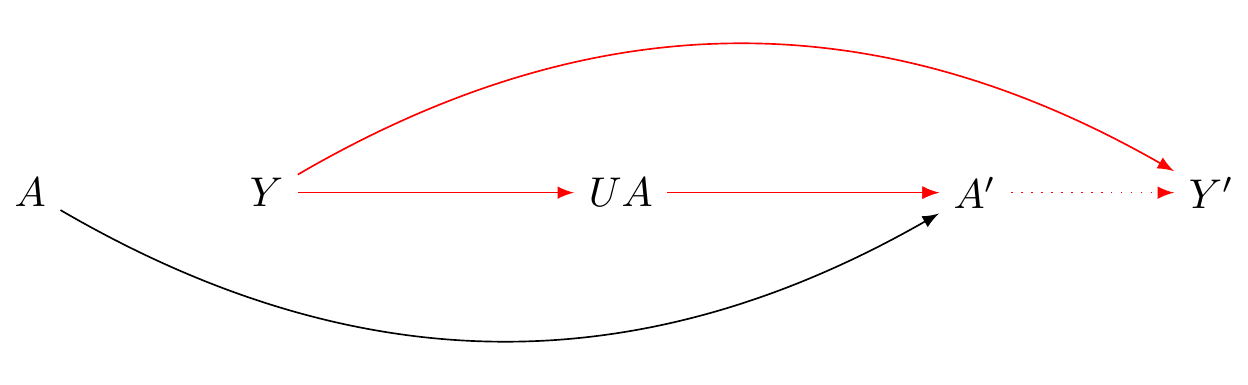
\includegraphics[width=1\textwidth,height=\textheight]{test-again_files/figure-pdf/fig-dag-measure-selection-0-1.pdf}

}

\caption{\label{fig-dag-measure-selection-0}Figure X illustrates the
impact of measurement error on the inferred causal relationship between
an exposure (A) and an outcome (Y). Both A and Y are assumed to be
measured without error. However, a confounder (L) is measured with
error, represented as L'. This error introduces a biasing path A - L -
Y, depicted in red. The potential for bias between A and Y, shown as a
red dotted path, is opened up due to this error in confounder
measurement.}

\end{figure}

Figure~\ref{fig-dag-measure-selection} reveals the structure of bias is
such post-outcome adjustment is needed to mitigate or remove measurement
bias when the outcome has caused it. Suppose our interest is again in
quantifying the effect of beliefs in big Gods on social complexity.
Suppose that socially complex societies re-write history removing trace
of beliefs in lesser Gods. Suppose that such traces are nevertheless
recoverable from linguistic variation.

\begin{figure}

{\centering 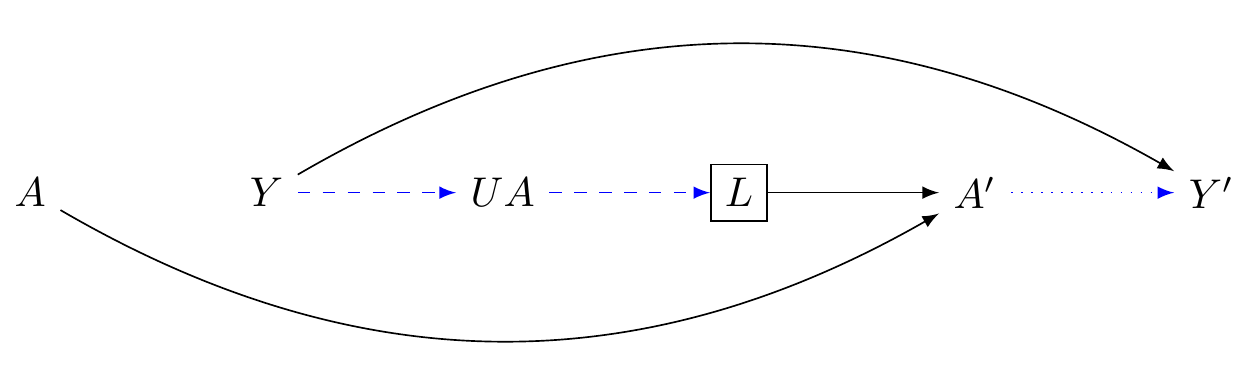
\includegraphics[width=1\textwidth,height=\textheight]{test-again_files/figure-pdf/fig-dag-measure-selection-1.pdf}

}

\caption{\label{fig-dag-measure-selection}Causal diagram reveals how
improved measures diminish bias. Blue doted arrows denote paths of
diminishing the effect of measurement error bias created because by
recovering measures of the distorted exposure (echoes of the silenced).}

\end{figure}

\hypertarget{refs}{}
\begin{CSLReferences}{1}{0}
\leavevmode\vadjust pre{\hypertarget{ref-mathur2018}{}}%
Mathur, Maya B, Peng Ding, Corinne A Riddell, and Tyler J VanderWeele.
2018. {``Website and r Package for Computing e-Values.''}
\emph{Epidemiology (Cambridge, Mass.)} 29 (5): e45.

\end{CSLReferences}



\end{document}
